
\chapter{Project Management}

\section{Gantt Chart}

\begin{figure}[ht]
  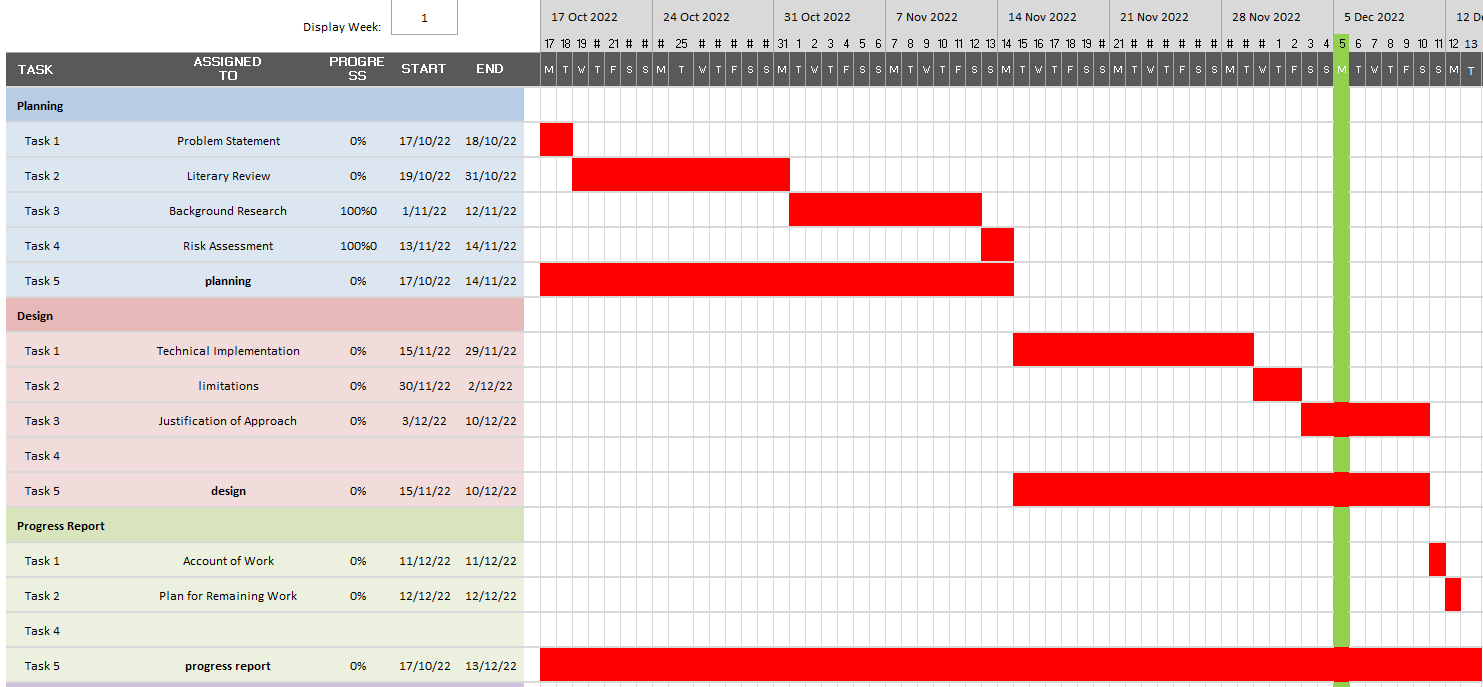
\includegraphics[width=\textwidth]{diagrams/gantt-chart-1.png}
  \caption{\textit{A Gantt chart for my work up until the progress report.}}
\end{figure}

% \begin{figure}[ht]
%   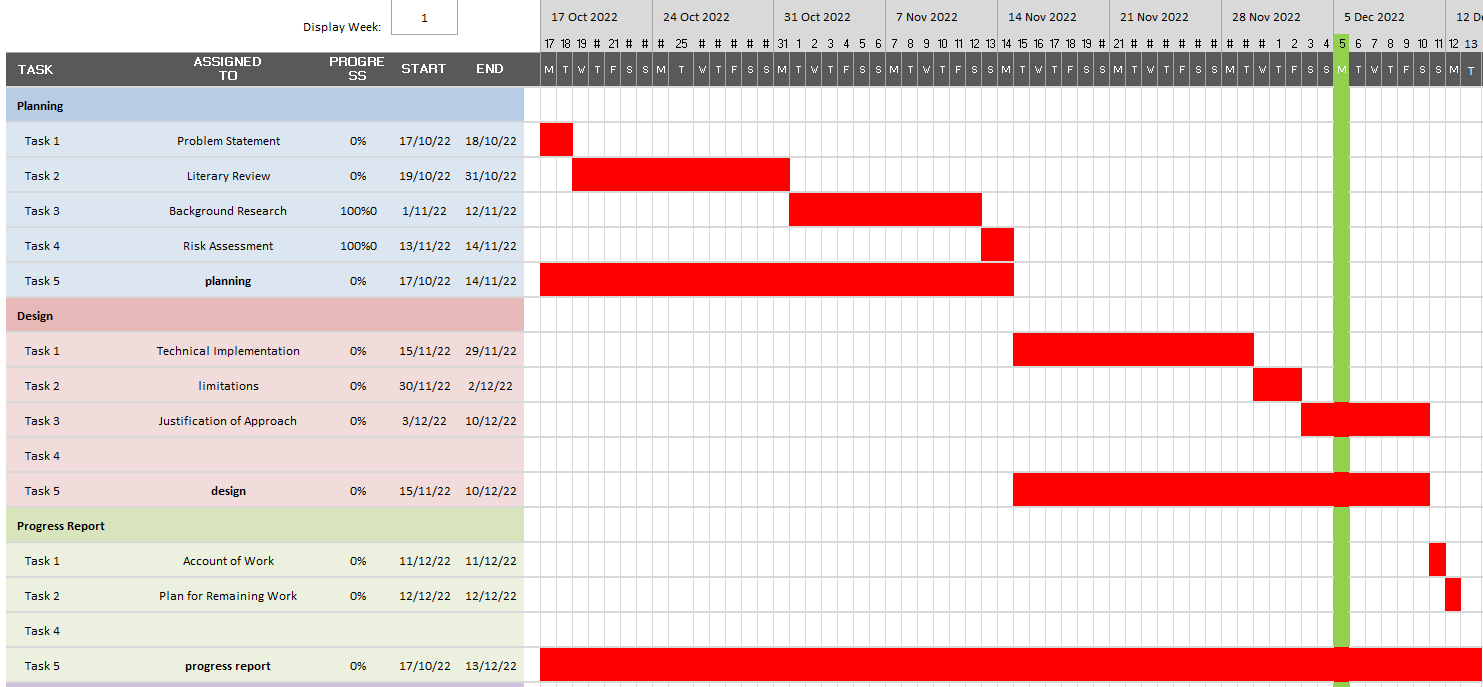
\includegraphics[width=\textwidth]{diagrams/gantt-chart-1.png}
%   \caption{\textit{A Gantt chart for my work by the handin of the progress report.}}
% \end{figure}

\section{Risk Assessment}

\begin{longtable}[ht]{ p{.2\textwidth} p{0.06\textwidth}  p{0.06\textwidth} p{0.06\textwidth} p{0.5\textwidth}}
  \toprule
  \textbf{Risk}
   & \textbf{Loss}
   & \textbf{Prob}
   & \textbf{Risk}
   & \textbf{Mitigation}
  %
  \\\midrule\midrule
  Laptop damaged or lost
   & 3
   & 1
   & \cellcolor{orange!50} 5
   & All work is stored using version control and periodic backups will be
  made and stored locally and in cloud storage. I have other devices that
  could be used to continue development.
  %
  \x
  Difficulty with blockchain development
   & 2
   & 3
   & \cellcolor{orange!50} 6
   & I will seek advice from my supervisor about how to tackle certain problems
  and if necessary, what aspects of my project I should change.
  %
  \x
  The application is not finished
   & 1
   & 3
   & \cellcolor{green!30} 3
   & Using agile development will ensure that I will at least have a minimal
  working application. If I feel that I am running out of time, I will focus
  on expanding test cases and improving the write-up.
  %
  \x
  No suitable large scale test environment
   & 2
   & 5
   & \cellcolor{red!40} 10
   & I do not have the infrastructure to test this project on a large network,
  however small scale tests will be possible.
  %
  \x
  Personal illness
  & 3
  & 2
  & \cellcolor{orange!50} 6
  & Depending on the amount of lost time, I may have to not complete some of the SHOULD or COULD requirements.
  \\\bottomrule\bottomrule
  \\\caption{\textit{The risk assessment of this project.}}
  \label{tab:risk assessment}
\end{longtable}